%-*- coding: utf-8 -*-
\subsection{Génération automatique des menus}
\begin{figure}[H]
\label{MenuGen}
  \centering
      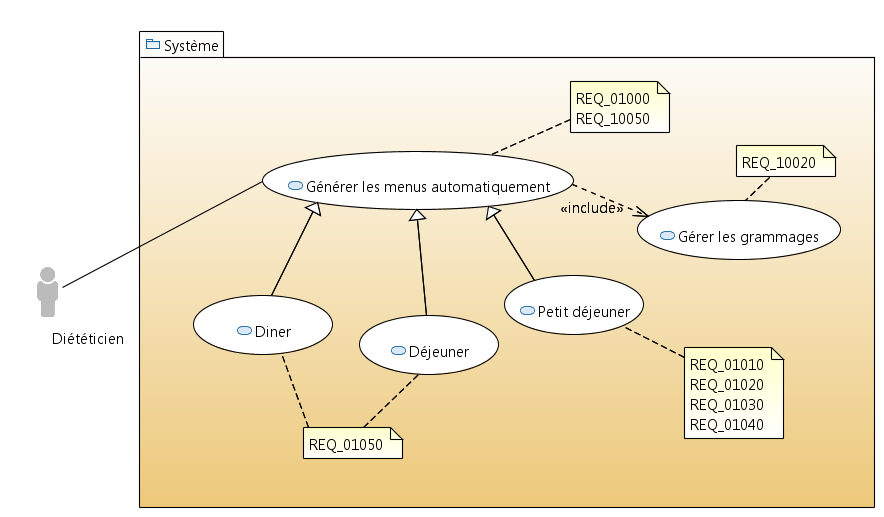
\includegraphics[width=1.00\textwidth]{../../CasDUtilisations/MenuGen/UseCase_Diagram} %
\caption{Génération automatique des menus}
\end{figure}

\begin{description}
\item[Nom:] Génération automatique des menus.
\item[ID:] REQ\_01000, REQ\_10020, REQ\_10050, REQ\_01010, REQ\_01020, REQ\_01030, REQ\_01040, REQ\_01050.
\item[Description:] Permet la génération automatique des menus.
\item[Acteurs:] Diététiciens.
\item[Pré-Conditions:] Le diététicien s'est connecté au système.
\item[Scénario principal:] Le diététicien sélectionne le groupe de patients pour lequel il veut générer les menus, ensuite il lance la génération automatique.
\item[Post-Conditions:] Les menus sont générés.
\item[Scénario alternatif:] Aucun.
\end{description}
